%% bare_conf_compsoc.tex
%% V1.4b
%% 2015/08/26
%% by Michael Shell
%% See:
%% http://www.michaelshell.org/
%% for current contact information.
%%
%% This is a skeleton file demonstrating the use of IEEEtran.cls
%% (requires IEEEtran.cls version 1.8b or later) with an IEEE Computer
%% Society conference paper.
%%
%% Support sites:
%% http://www.michaelshell.org/tex/ieeetran/
%% http://www.ctan.org/pkg/ieeetran
%% and
%% http://www.ieee.org/

%%*************************************************************************
%% Legal Notice:
%% This code is offered as-is without any warranty either expressed or
%% implied; without even the implied warranty of MERCHANTABILITY or
%% FITNESS FOR A PARTICULAR PURPOSE!
%% User assumes all risk.
%% In no event shall the IEEE or any contributor to this code be liable for
%% any damages or losses, including, but not limited to, incidental,
%% consequential, or any other damages, resulting from the use or misuse
%% of any information contained here.
%%
%% All comments are the opinions of their respective authors and are not
%% necessarily endorsed by the IEEE.
%%
%% This work is distributed under the LaTeX Project Public License (LPPL)
%% ( http://www.latex-project.org/ ) version 1.3, and may be freely used,
%% distributed and modified. A copy of the LPPL, version 1.3, is included
%% in the base LaTeX documentation of all distributions of LaTeX released
%% 2003/12/01 or later.
%% Retain all contribution notices and credits.
%% ** Modified files should be clearly indicated as such, including  **
%% ** renaming them and changing author support contact information. **
%%*************************************************************************


% *** Authors should verify (and, if needed, correct) their LaTeX system  ***
% *** with the testflow diagnostic prior to trusting their LaTeX platform ***
% *** with production work. The IEEE's font choices and paper sizes can   ***
% *** trigger bugs that do not appear when using other class files.       ***                          ***
% The testflow support page is at:
% http://www.michaelshell.org/tex/testflow/



\documentclass[conference,compsoc]{IEEEtran}
% Some/most Computer Society conferences require the compsoc mode option,
% but others may want the standard conference format.
%
% If IEEEtran.cls has not been installed into the LaTeX system files,
% manually specify the path to it like:
% \documentclass[conference,compsoc]{../sty/IEEEtran}





% Some very useful LaTeX packages include:
% (uncomment the ones you want to load)


% *** MISC UTILITY PACKAGES ***
%
%\usepackage{ifpdf}
% Heiko Oberdiek's ifpdf.sty is very useful if you need conditional
% compilation based on whether the output is pdf or dvi.
% usage:
% \ifpdf
%   % pdf code
% \else
%   % dvi code
% \fi
% The latest version of ifpdf.sty can be obtained from:
% http://www.ctan.org/pkg/ifpdf
% Also, note that IEEEtran.cls V1.7 and later provides a builtin
% \ifCLASSINFOpdf conditional that works the same way.
% When switching from latex to pdflatex and vice-versa, the compiler may
% have to be run twice to clear warning/error messages.






% *** CITATION PACKAGES ***
%
\ifCLASSOPTIONcompsoc
  % IEEE Computer Society needs nocompress option
  % requires cite.sty v4.0 or later (November 2003)
  \usepackage[nocompress]{cite}
\else
  % normal IEEE
  \usepackage{cite}
\fi
% cite.sty was written by Donald Arseneau
% V1.6 and later of IEEEtran pre-defines the format of the cite.sty package
% \cite{} output to follow that of the IEEE. Loading the cite package will
% result in citation numbers being automatically sorted and properly
% "compressed/ranged". e.g., [1], [9], [2], [7], [5], [6] without using
% cite.sty will become [1], [2], [5]--[7], [9] using cite.sty. cite.sty's
% \cite will automatically add leading space, if needed. Use cite.sty's
% noadjust option (cite.sty V3.8 and later) if you want to turn this off
% such as if a citation ever needs to be enclosed in parenthesis.
% cite.sty is already installed on most LaTeX systems. Be sure and use
% version 5.0 (2009-03-20) and later if using hyperref.sty.
% The latest version can be obtained at:
% http://www.ctan.org/pkg/cite
% The documentation is contained in the cite.sty file itself.
%
% Note that some packages require special options to format as the Computer
% Society requires. In particular, Computer Society  papers do not use
% compressed citation ranges as is done in typical IEEE papers
% (e.g., [1]-[4]). Instead, they list every citation separately in order
% (e.g., [1], [2], [3], [4]). To get the latter we need to load the cite
% package with the nocompress option which is supported by cite.sty v4.0
% and later.


%\usepackage[outdir=./plots/]{epstopdf}
\usepackage[pdftex]{graphicx}

% *** GRAPHICS RELATED PACKAGES ***
%
%\ifCLASSINFOpdf
%  \usepackage[pdftex]{graphicx}
  % declare the path(s) where your graphic files are
  % \graphicspath{{../pdf/}{../jpeg/}}
  % and their extensions so you won't have to specify these with
  % every instance of \includegraphics
  % \DeclareGraphicsExtensions{.pdf,.jpeg,.png}
%\else
  % or other class option (dvipsone, dvipdf, if not using dvips). graphicx
  % will default to the driver specified in the system graphics.cfg if no
  % driver is specified.
  % \usepackage[dvips]{graphicx}
  % declare the path(s) where your graphic files are
  % \graphicspath{{../eps/}}
  % and their extensions so you won't have to specify these with
  % every instance of \includegraphics
  % \DeclareGraphicsExtensions{.eps}
%\fi
% graphicx was written by David Carlisle and Sebastian Rahtz. It is
% required if you want graphics, photos, etc. graphicx.sty is already
% installed on most LaTeX systems. The latest version and documentation
% can be obtained at:
% http://www.ctan.org/pkg/graphicx
% Another good source of documentation is "Using Imported Graphics in
% LaTeX2e" by Keith Reckdahl which can be found at:
% http://www.ctan.org/pkg/epslatex
%
% latex, and pdflatex in dvi mode, support graphics in encapsulated
% postscript (.eps) format. pdflatex in pdf mode supports graphics
% in .pdf, .jpeg, .png and .mps (metapost) formats. Users should ensure
% that all non-photo figures use a vector format (.eps, .pdf, .mps) and
% not a bitmapped formats (.jpeg, .png). The IEEE frowns on bitmapped formats
% which can result in "jaggedy"/blurry rendering of lines and letters as
% well as large increases in file sizes.
%
% You can find documentation about the pdfTeX application at:
% http://www.tug.org/applications/pdftex





% *** MATH PACKAGES ***
%
%\usepackage{amsmath}
% A popular package from the American Mathematical Society that provides
% many useful and powerful commands for dealing with mathematics.
%
% Note that the amsmath package sets \interdisplaylinepenalty to 10000
% thus preventing page breaks from occurring within multiline equations. Use:
%\interdisplaylinepenalty=2500
% after loading amsmath to restore such page breaks as IEEEtran.cls normally
% does. amsmath.sty is already installed on most LaTeX systems. The latest
% version and documentation can be obtained at:
% http://www.ctan.org/pkg/amsmath





% *** SPECIALIZED LIST PACKAGES ***
%
%\usepackage{algorithmic}
% algorithmic.sty was written by Peter Williams and Rogerio Brito.
% This package provides an algorithmic environment fo describing algorithms.
% You can use the algorithmic environment in-text or within a figure
% environment to provide for a floating algorithm. Do NOT use the algorithm
% floating environment provided by algorithm.sty (by the same authors) or
% algorithm2e.sty (by Christophe Fiorio) as the IEEE does not use dedicated
% algorithm float types and packages that provide these will not provide
% correct IEEE style captions. The latest version and documentation of
% algorithmic.sty can be obtained at:
% http://www.ctan.org/pkg/algorithms
% Also of interest may be the (relatively newer and more customizable)
% algorithmicx.sty package by Szasz Janos:
% http://www.ctan.org/pkg/algorithmicx




% *** ALIGNMENT PACKAGES ***
%
\usepackage{array}
% Frank Mittelbach's and David Carlisle's array.sty patches and improves
% the standard LaTeX2e array and tabular environments to provide better
% appearance and additional user controls. As the default LaTeX2e table
% generation code is lacking to the point of almost being broken with
% respect to the quality of the end results, all users are strongly
% advised to use an enhanced (at the very least that provided by array.sty)
% set of table tools. array.sty is already installed on most systems. The
% latest version and documentation can be obtained at:
% http://www.ctan.org/pkg/array


% IEEEtran contains the IEEEeqnarray family of commands that can be used to
% generate multiline equations as well as matrices, tables, etc., of high
% quality.




% *** SUBFIGURE PACKAGES ***
%\ifCLASSOPTIONcompsoc
%  \usepackage[caption=false,font=footnotesize,labelfont=sf,textfont=sf]{subfig}
%\else
%  \usepackage[caption=false,font=footnotesize]{subfig}
%\fi
% subfig.sty, written by Steven Douglas Cochran, is the modern replacement
% for subfigure.sty, the latter of which is no longer maintained and is
% incompatible with some LaTeX packages including fixltx2e. However,
% subfig.sty requires and automatically loads Axel Sommerfeldt's caption.sty
% which will override IEEEtran.cls' handling of captions and this will result
% in non-IEEE style figure/table captions. To prevent this problem, be sure
% and invoke subfig.sty's "caption=false" package option (available since
% subfig.sty version 1.3, 2005/06/28) as this is will preserve IEEEtran.cls
% handling of captions.
% Note that the Computer Society format requires a sans serif font rather
% than the serif font used in traditional IEEE formatting and thus the need
% to invoke different subfig.sty package options depending on whether
% compsoc mode has been enabled.
%
% The latest version and documentation of subfig.sty can be obtained at:
% http://www.ctan.org/pkg/subfig




% *** FLOAT PACKAGES ***
%
%\usepackage{fixltx2e}
% fixltx2e, the successor to the earlier fix2col.sty, was written by
% Frank Mittelbach and David Carlisle. This package corrects a few problems
% in the LaTeX2e kernel, the most notable of which is that in current
% LaTeX2e releases, the ordering of single and double column floats is not
% guaranteed to be preserved. Thus, an unpatched LaTeX2e can allow a
% single column figure to be placed prior to an earlier double column
% figure.
% Be aware that LaTeX2e kernels dated 2015 and later have fixltx2e.sty's
% corrections already built into the system in which case a warning will
% be issued if an attempt is made to load fixltx2e.sty as it is no longer
% needed.
% The latest version and documentation can be found at:
% http://www.ctan.org/pkg/fixltx2e


%\usepackage{stfloats}
% stfloats.sty was written by Sigitas Tolusis. This package gives LaTeX2e
% the ability to do double column floats at the bottom of the page as well
% as the top. (e.g., "\begin{figure*}[!b]" is not normally possible in
% LaTeX2e). It also provides a command:
%\fnbelowfloat
% to enable the placement of footnotes below bottom floats (the standard
% LaTeX2e kernel puts them above bottom floats). This is an invasive package
% which rewrites many portions of the LaTeX2e float routines. It may not work
% with other packages that modify the LaTeX2e float routines. The latest
% version and documentation can be obtained at:
% http://www.ctan.org/pkg/stfloats
% Do not use the stfloats baselinefloat ability as the IEEE does not allow
% \baselineskip to stretch. Authors submitting work to the IEEE should note
% that the IEEE rarely uses double column equations and that authors should try
% to avoid such use. Do not be tempted to use the cuted.sty or midfloat.sty
% packages (also by Sigitas Tolusis) as the IEEE does not format its papers in
% such ways.
% Do not attempt to use stfloats with fixltx2e as they are incompatible.
% Instead, use Morten Hogholm'a dblfloatfix which combines the features
% of both fixltx2e and stfloats:
%
% \usepackage{dblfloatfix}
% The latest version can be found at:
% http://www.ctan.org/pkg/dblfloatfix




% *** PDF, URL AND HYPERLINK PACKAGES ***
%
%\usepackage{url}
% url.sty was written by Donald Arseneau. It provides better support for
% handling and breaking URLs. url.sty is already installed on most LaTeX
% systems. The latest version and documentation can be obtained at:
% http://www.ctan.org/pkg/url
% Basically, \url{my_url_here}.




% *** Do not adjust lengths that control margins, column widths, etc. ***
% *** Do not use packages that alter fonts (such as pslatex).         ***
% There should be no need to do such things with IEEEtran.cls V1.6 and later.
% (Unless specifically asked to do so by the journal or conference you plan
% to submit to, of course. )


\usepackage[utf8]{inputenc}

% correct bad hyphenation here
\hyphenation{op-tical net-works semi-conduc-tor}


\begin{document}
%
% paper title
% Titles are generally capitalized except for words such as a, an, and, as,
% at, but, by, for, in, nor, of, on, or, the, to and up, which are usually
% not capitalized unless they are the first or last word of the title.
% Linebreaks \\ can be used within to get better formatting as desired.
% Do not put math or special symbols in the title.
\title{Concurrency and Parallelism\\ Cilk$^+$ Parallel Patterns Implementation }


%\institute{DI - FCT - NOVA University of Lisbon}

% author names and affiliations
% use a multiple column layout for up to three different
% affiliations
\author{\IEEEauthorblockN{André Rosa}
\IEEEauthorblockA{%Computer Science Department\\
%FCT-UNL\\
%Almada, Setúbal\\
48043\\
af.rosa@campus.fct.unl.pt}
\and
\IEEEauthorblockN{João Geraldo}
\IEEEauthorblockA{%Computer Science Department\\
%FCT-UNL\\
%Almada, Setúbal\\
49543\\
j.geraldo@campus.fct.unl.pt}
\and
\IEEEauthorblockN{Rúben Silva}
\IEEEauthorblockA{%Computer Science Department\\
%FCT-UNL\\
%Almada, Setúbal\\
47134\\
rfc.silva@campus.fct.unl.pt}}

% conference papers do not typically use \thanks and this command
% is locked out in conference mode. If really needed, such as for
% the acknowledgment of grants, issue a \IEEEoverridecommandlockouts
% after \documentclass

% for over three affiliations, or if they all won't fit within the width
% of the page (and note that there is less available width in this regard for
% compsoc conferences compared to traditional conferences), use this
% alternative format:
%
%\author{\IEEEauthorblockN{Michael Shell\IEEEauthorrefmark{1},
%Homer Simpson\IEEEauthorrefmark{2},
%James Kirk\IEEEauthorrefmark{3},
%Montgomery Scott\IEEEauthorrefmark{3} and
%Eldon Tyrell\IEEEauthorrefmark{4}}
%\IEEEauthorblockA{\IEEEauthorrefmark{1}School of Electrical and Computer Engineering\\
%Georgia Institute of Technology,
%Atlanta, Georgia 30332--0250\\ Email: see http://www.michaelshell.org/contact.html}
%\IEEEauthorblockA{\IEEEauthorrefmark{2}Twentieth Century Fox, Springfield, USA\\
%Email: homer@thesimpsons.com}
%\IEEEauthorblockA{\IEEEauthorrefmark{3}Starfleet Academy, San Francisco, California 96678-2391\\
%Telephone: (800) 555--1212, Fax: (888) 555--1212}
%\IEEEauthorblockA{\IEEEauthorrefmark{4}Tyrell Inc., 123 Replicant Street, Los Angeles, California 90210--4321}}

% make the title area
\maketitle


% use for special paper notices
%\IEEEspecialpapernotice{(Invited Paper)}


%\markboth{Journal of \LaTeX\ Class Files,~Vol.~14, No.~8, August~2015}%
%{Shell \MakeLowercase{\textit{et al.}}: Bare Demo of IEEEtran.cls for Computer Society Journals}

% As a general rule, do not put math, special symbols or citations
% in the abstract
%\IEEEtitleabstractindextext{
\begin{abstract}

In recent years, the parallel computation paradigm has emerged as a consequence to the explosive increase in the amount of data available to process  and the shift in processor's architecture evolution to integrate parallel functionalities, such as multiple cores, hardware threads and vector operations.
Therefore, in order to fully utilize the potential of parallel hardware and more efficiently process large amounts of data, it is imperative to design algorithms that explore these functionalities.

However, designing algorithms on top of them can sometimes be a difficult and complex task, due to very complex nature of parallel computations and by the fact that parallel hardware functionalities exist as low level primitives, being sometimes platform dependent.
Thus, parallel functions and libraries can provide an easy and generic way to better utilize these resources, when available.
Therefore, we developed a library, that implements some of the most well known parallel patterns, allowing the composition of algorithms and, at the same time, can easily be integrated with any already existing sequential program, to improve its efficiency. In order to be able to use the library in a vast amount of use cases, the  pattern implementations are independent both from the data types they are manipulating and the parallel functionalities provided by each specific hardware platform.

In the implementation of each parallel pattern, we sought to maximize the amount of parallel slack. We also prioritized the decrease in execution time when implementing the various patterns, which for some of them meant increasing the amount of reserved memory to ensure better data locality and cache usage. Certain patterns were implemented in a generic, parameterizable way, which allows for flexibility in the distribution of work regarding the computational weight of the operations and the size of the data types being manipulated, resulting in the most efficient execution.

Finally, we conducted a preliminary experimental evaluation on the performance of the different implemented alternatives, comparing them with their corresponding sequential counterparts, that showed noticeable gains in performance for several of the parallel patterns.

\end{abstract}

\IEEEpeerreviewmaketitle

\begin{IEEEkeywords}
Parallel Algorithms, Cilk$^+$
\end{IEEEkeywords}%}


\section{Introduction}

Parallel computing is a type of computation in which several independent tasks are executed simultaneously. In recent years, the parallel computation paradigm has grown in relevance as a consequence of two modern trends: the amount of data to process and the architectural evolution of processors.
In the one hand, the explosive increase in the amount of data produced every day \cite{mcafee2012big}, lead to a demand of more scalabel and efficient data processing algorithms. %requiring more computational power to process and analyze it at useful rates.
On the other hand, due to the fact that single-core processors are reaching the physical limits of improvement through increasing its clock frequency and shrinking of its components, to decrease the communication time between them, a revolution happened in the processor's architecture design. Consequently, processors' architecture evolution switched to insert parallel functionalities, such as having multiple cores and hardware threads as well as supporting vector operations, that allow the simultaneous execution of processes and parallel manipulation of multiple data.

For these reasons, it is imperative that algorithms are designed with parallelism in mind, in order to fully take advantage of the potential of the parallel hardware they are being executed on, to process large amounts of data more efficiently, and at the same time provide scalability, to be prepared to the evolution of both the hardware and the amount of data produced.

However, the conception of parallel algorithms can be a very difficult and complex task due to the very complex nature of parallel computations, and by the fact that parallel hardware functionalities exist as low level primitives, being sometimes platform dependent and highly heterogeneous, i.e., not all the processors provide vector operations and hardware threads, and the number of cores may vary greatly, even within the same manufacturer: take Intel as an example - Intel's i7 lineup has chips with only 2 cores up to chips with a whopping 16 cores. Parallel functions and libraries provide an easy and generic way to better utilize parallel hardware resources, when available.

%Through the abstraction provided by those libraries, it is possible to write hardware-independent algorithms.
Simultaneously, just like sequential algorithms, the parallel ones also have a set of a specific recurring configuration of computations and data accesses. These configurations are called parallel patterns \cite{mccool2010structured} and they can help conceive parallel algorithms, serving as building blocks that can be glued together to produce an algorithm.% Thus, a parallel algorithm can be seen as a composition of these parallel patterns.

On that account, we designed and implemented a library that contains some of the most well known parallel patterns, providing at the same time abstraction from the available hardware resources. To be able to use it in a vast amount of use cases, these implementations were also designed to be independent from the data types they are manipulating.
Thus, this library provides an easy way to construct parallel programs as well as integrate it with little effort on already-built sequential programs, making use of the available hardware parallel functionalities and consequently improve its efficiency.
To implement those patterns, we resorted to Intel's Cilk$^+$ \cite{robison2012cilk}, a C/C++ extension that support data and task parallelism.
In the implementation of each parallel pattern, we sought to maximize the amount of parallel slack i.e. excess of potential parallelism versus actual amount of hardware parallelism. This approach guarantees an efficient use of hardware resources, since different machines will be able to execute the parallel patterns with varying amounts of parallelism. We prioritized the decrease in execution time of the implemented patterns, which for some of them meant increasing the amount of reserved memory to ensure better data locality and cache usage. Certain patterns were implemented in a generic, parameterizable way, which allows for flexibility in the distribution of work regarding the computational weight of the operations and the size of the data types being manipulated, resulting in the most efficient execution.

The remaining of this report is structured as follows: at Section~\ref{Architecture} we present the architecture of the algorithms and at Section~\ref{Implementation} we discuss their relevant implementation details. The settings of the experimental evaluation, along with a discussion about the results obtained and present possible explanations for the differences in computational performance for the various patterns, that are presented in Section~\ref{Experimental_Eval}. Lastly, we conclude this report with the conclusions, at Section~\ref{Conclusion}.

\section{Architecture} \label{Architecture}

In this Section, we describe the architecture of each of the implement patterns in our library: Map, Reduce, Scan, Pack, Split, Gather, Scatter, Pipeline and Farm. [citações para os patterns]

\subsection{Map}
The Map pattern consists on the independent application of the same function (or worker) to every element of a collection. This function needs to be pure, i.e., not have side effects in order to be parallelizable. As the applications of the function are independent from one another, they can be executed in parallel.
However, sometimes the computational weight of the function might be too small in comparison to the overhead of parallelizing their execution, leading to worst results than utilizing the sequential version. Thus, to overcome this problem, the elements of the collection can be grouped in batches, which are processed in parallel, and, within each batch, their elements are processed sequentially. The size of each batch is called \emph{Grain Size} and the separation in groups is called \emph{Granularity}. We implement our map following that behavior.

\subsection{Reduce}
The Reduce pattern consists on applying a pairwise associative operation (e.g. Add, Multiply) to all the elements of a collection, producing a single element. Since the operation is associative, multiple applications (to different elements) can be done in parallel. The execution of the parallel version of these pattern produces a binary tree, where the child nodes are the operands and the parent is the result of the operation, being that the result of reduce corresponds to the root of this tree.

In our library, we decided to implemented two versions of reduce: (regular) reduce and tiled reduce. In regular reduce, the elements of the collection are paired and the worker (operator) is applied in parallel to each pair. This process is repeated to their results until there is only one element, the reduce result.
However, the weight of operator may be too small compared to the parallelization overhead, that it does not pay to use the parallel version.
Thus, we decided to implement the alternative version, tiled reduce, which groups several elements of the collection in a tile, instead of only two. This tiles are then processed in parallel, being that for each one, a sequential version of reduce is executed.

[Secalhar explicar mais em detalhe a nossa implementação]

%problem of semi
%-
%associative operations
%such as floating point arithmetic.

%Explicar que quisemos aumentar oa máximo parallel slack e por isso quando o array de ouptu é grande este é continuamente dividido na versaõ tiled até ter um tamanho minimo. Formando uma árvore n-ária em vez de binária.
%Explicar a técnica dos dois arrays para fazer a árvore de execução mas sem a armazenar toda em memória e poupar espaço sem ter apontadores para os pais e filhos, etc.

\subsection{Scan}

The Scan pattern is very similar to the Reduce pattern,
with the difference that it returns a sequence, with the results of all the intermediate operations, and not just the result of the last operation.
The order of the sequence must be the same as the order of the sequential version's result.

We decided to implement this version of Scan \cite{ladner1980parallel}, that is composed by two phases.
In the first, it builds a tree, in a bottom-up approach, similarly to reduce, where the nodes are the results of the intermediate operations are computed pairwise, with the exception of the leafs, that correspond to input elements. The root of these tree corresponds to the result of applying the operator to all the input's elements, i.e., it's the same as the reduce value.
In the second phase, it traverses the tree, in a top-down approach, passing to the left child of each node, the value inherited from its parent (the neutral element of the operation in the case of the root) and to the right child the result of applying the operator to the value inherited with the result of the intermediate computation of its left brother. In it reaches the leaves, the value to insert in the output collection corresponds to applying the operator to the inherited value and its own intermediate value.
One important aspect of this algorithm is that the total work to be done is higher, having complexity O(log n), however the the value of the span decreases, to O(log n).

This implementation has work O(n) but its span is only O (log n).

\subsection{Pack}

The Pack pattern consists on removing elements from a collection, keeping the remaining elements at contiguous positions, i.e., without unused space between them. The elements to remove (or to keep) are identified through a binary mask or a filter function function. In this pattern, the order of the elements is the same as their relative position in the input.

This pattern is generally used to eliminate wasted space in a sparse collection and to handle variable-rate output from a map (or other patterns), where the worker is allowed to either keep or discard its outputs.
We considered designing our own algorithm to implement Pack, however, the version proposed in the classes was more efficient, and thus we opted to implement that instead. That version resorts to Scan to compute the sum of the mask elements, originating the bitsum. That sequence, gives, for each true element on the mask, the corresponding input's element position in the output collection. Then, a map is applied to the bitsum with a worker that for each true element of the mask, inserts the corresponding element of the input collection into the output collection, in the position defined by the corresponding bitsum.

This implementation have work O(n) and span O(log n). [melhorar isto]

\subsection{Split}

The Split\footnote[1]{Optional Extra Pattern} pattern is a variant of pack which does not discard elements and instead packs them after the last element of the elements whose mask value was true, i.e., splits the true elements to one side of the collection and the falses to the other.
In this pattern, similarly to pack, the the order of the elements, within each output segment, is the same as their relative position in the input, in other words, it's a "stable" reordering, being that output size is always exactly the same size as the input's.
Split can obviously be implemented by running pack twice and then merging the results. However, because this wouldn't be the most efficient implementation, we developed a more direct algorithm that improves latency. First, it computes the inverse of the mask, turning the falses into trues and vice-versa. Then, parallel executes two scans, one on the original mask and another on the inverted mask, similarly to pack, producing positiveBitsum and negativeBitsum collections respectively. Afterwards, waits for the termination of the scans and then applies a single map across the input collection, with a worker that, for each element, if it's true on the original mask, insert it in the output collection, at the position given by positiveBitsum, else insert it in the output collection, at the position given by negativeBitsum plus an offset that corresponds to the amount of elements that are true in the mask and this value is given by the value on the last element of the positiveBitsum.

\subsection{Gather}

The Gather pattern takes a collection (input) and a sequence of indices (filter)  then it produces a collection (output)
composed by the elements of the input collection in a way that the output[i] = input[ filter[ i ] ].
Since only multiple reads can happen on the same element simultaneously, then each element of the index sequence can be processed in parallel.
We implemented this pattern resorting to the Map pattern, where the worker function corresponds to reading the element at the given index from the input collection and writing it in the corresponding slot in the sequence.

\subsection{Scatter}

The Scatter pattern is the inverse of gather. It also takes an input collection (input) and a sequence of indices (filter) in the previous collection and puts
 the element input[i] at index[i] in the output collection. There is a problem with this pattern that is if the index collection
 has repeated elements then data races occur.
  In our implementation, we left that verification to the user of the pattern because it would add too much weight
   to the operation and we think it should be a concern of the program that uses the function and not the function itself (pre-condition).
  We implemented this pattern resorting to map, where the worker copies the value in the position i of the input array to position index[i] in the output array.

[Está um bocado mal explicado]

\subsection{Pipeline}
The Pipeline pattern represents the sequential application of multiple operators (or stages) at the same element. Due to having multiple operators, they can be applied in parallel to different elements. However, having only one element at each stage can be too slow and thus, we implemented an alternative parallel version of pipeline - pipeline farm, that have multiple elements being processed at each stage in parallel and thus increase the throughput of the algorithm. This alternative version results from the combination of the Pipeline and Farm parallel patterns.

%However, for the same reasons as reduce, the weight of each operator might be too small compared to the parallel overhead that it's not worth to use the parallel version. Thus, we also developed an alternative version for pipeline - pipeline farm, that consists in group elements in batches, and process it seq [não sei que mais dizer]

\subsection{Farm}
The Farm pattern is very similar to Map with the constraint that the maximum amount of parallel operations is limited to the number of farms (parameter of the pattern). Thus, each job can be distributed evenly through all the farms and then processed sequentially in the respective farm.

\section{Implementation} \label{Implementation}

In this Section, we present some implementation details of our algorithms, that we found relevant.

In the Map pattern implementation, we would like to point out that we delegated the splitting of the source array into batches to the Cilk$^+$ runtime.
%, for that it takes into consideration the size, and the number of the elements to process.
We tried to make the batching separation ourselves, however, because we were getting poorer outcomes, and because we couldn't make assumptions on data types we were manipulating, and thus not know its size, we decided make use of Cilk$^+$'s automatic splitting.

%No map deixámos a separação em batches para o runtime do Cilk, que faz a separação automaticamente. Tentamos alterar os valores default mas obtivemos piores resultados e, visto que não podemos assumir com que tipos de dados estamos a lidar, achamos melhor deixar esta separação para o Cilk.


In the Reduce pattern implementation, to avoid data-races when trying to keep the intermediates results contiguous in memory (for faster sequential processing), we decided to use two intermediate arrays, one to read and another to write, that switch roles at each iteration ( level on the execution tree ) of reduce. This allowed to not keep all the intermediate results in memory, because they are only needed to compute the next level results, and at the same time improve the processing of each level by keeping all the elements contiguous and thus, increase the processing of the sequential version algorithm on each batch (or pair of elements in the case of regular reduce).

%Na nossa implementação do reduce, de forma a evitar dataraces e a manter os resultados intermédios contigous em memória, resolvemos utilizar dois arrays auxiliares, um para escrita e outro para leitura, que vão sendo alternados a cada iteração do reduce.

%Falar que o slpit não saõ 2 packs porque tinham de ser 1 depois do outro? ou isso é retardado?

\section{Experimental Evaluation} \label{Experimental_Eval}
In this Section we present an experimental evaluation of the implemented parallel algorithms, comparing their performance against their sequential version.

\subsection{Experimental Setting}

%To evaluate the performance of our parallel algorithms, we built a tester application that, for each algorithm, runs each of its versions (parallel, sequential and alternative, when there is one) one after the other a parameterizable amount of times, in order to compute the average of their results and thus filter the noise introduced by the ... . For each algorithm we measured its latency for multiple amount of jobs and its latency for a fixed amount of jobs, with variable computation work. In order to count the elapsed time between the start and finish of the algorithm, we resort to a system call [citar] that returns the amount of the process CPU time, and thus not counting the time when the process is interrupted by the OS's process scheduler, giving more accurate results for the latency. The units utilized are microseconds (us). We run the experiments on node9, a computer with 16 cores and .... .

To evaluate the performance of our parallel algorithms, we built a tester application that, for each algorithm, runs each of its versions: sequential, parallel and alternative, when there is one; and measure its latency, i.e., the elapsed time between the start and finish of the algorithm's version. For a given algorithm, it computes the latency for a sequence of job sizes, allowing us to measure the behavior of our solution regarding the input size. Each algorithm version for a given job amount, is run a parameterizable amount of times, in order to compute the average of their results and thus smooth the noise introduced by other processes and hardware details. The precision of the time measures are in the magnitude of microseconds (us), but the results are presented in seconds to improve readability.
Our experimental evaluation was executed in node9, a computer with 16 processors: Dual-Core AMD Opteron 8220 with 1000 MHz, Cache of 1024 Kb and
TLB size of 1024 4K pages; and 27 GB of RAM. The results of these experiments are presented in the following section.


\subsection{Experimental Results}

\begin{figure}[h!]
  \centering
  \setlength\tabcolsep{0.01pt}
  %\renewcommand{\arraystretch}{0.5}
  \begin{tabular}{cc}

    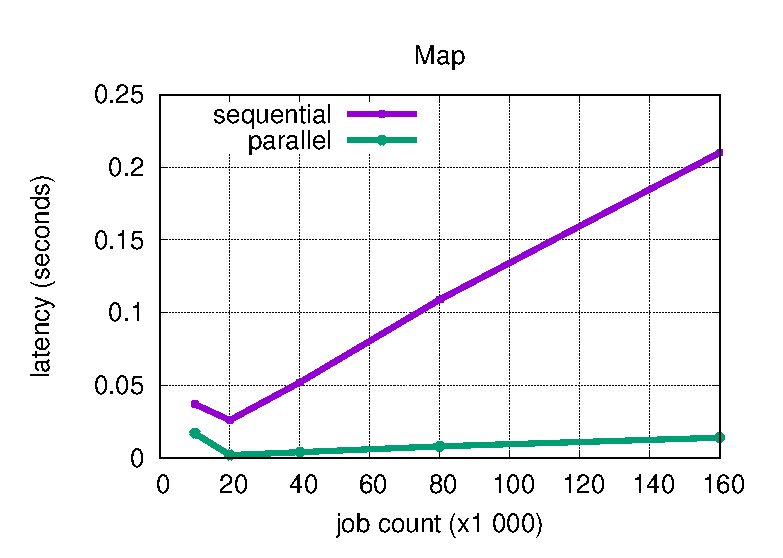
\includegraphics[width=0.265\textwidth]{plots/Map.eps} & 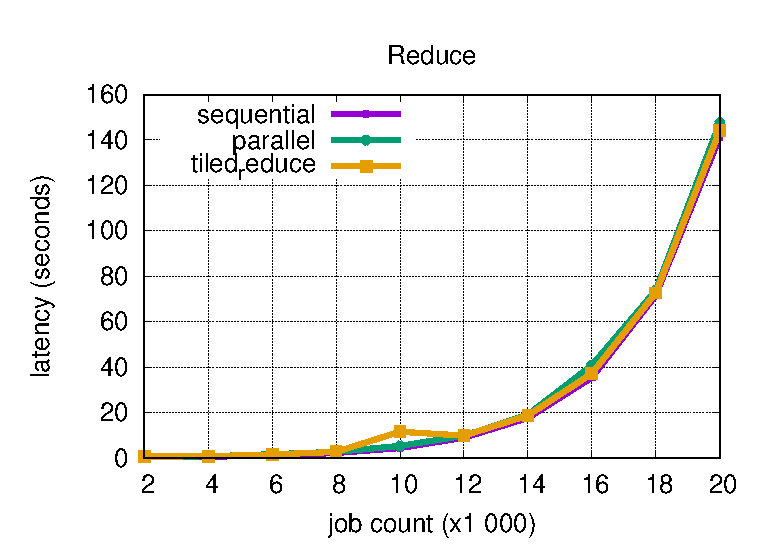
\includegraphics[width=0.265\textwidth]{plots/Reduce.eps}\\
    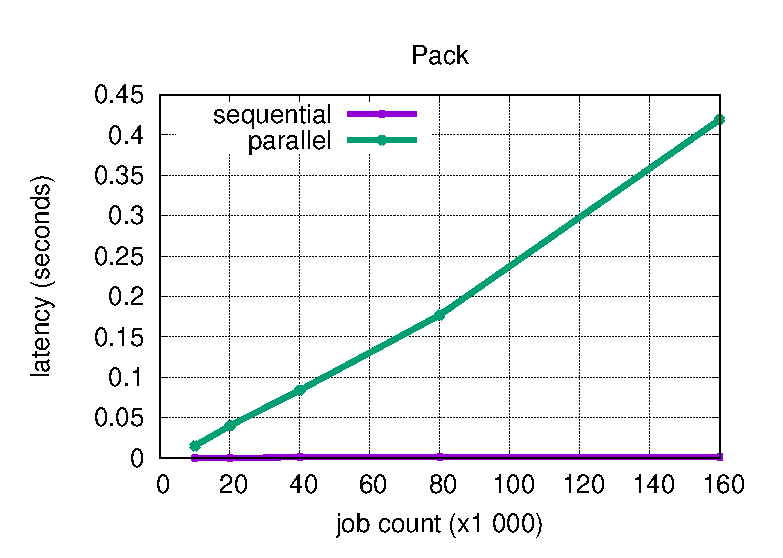
\includegraphics[width=0.265\textwidth]{plots/Pack.eps} & 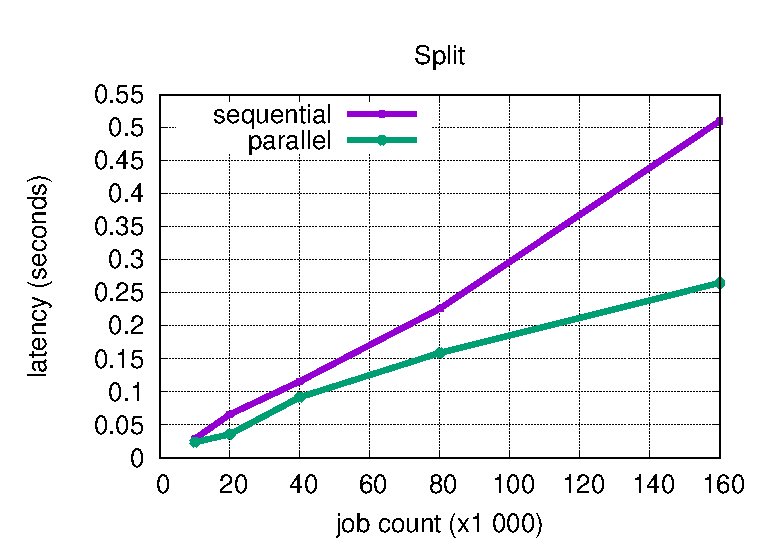
\includegraphics[width=0.265\textwidth]{plots/Split.eps}\\
    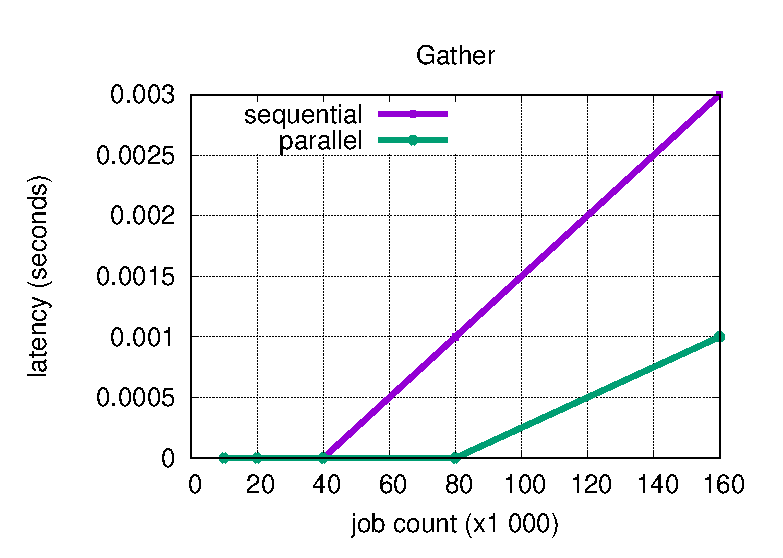
\includegraphics[width=0.265\textwidth]{plots/Gather.eps} & 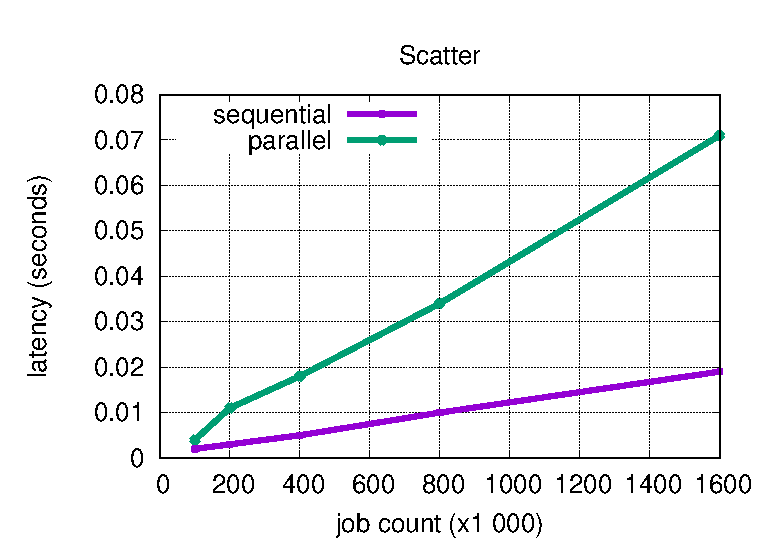
\includegraphics[width=0.265\textwidth]{plots/Scatter.eps}\\
    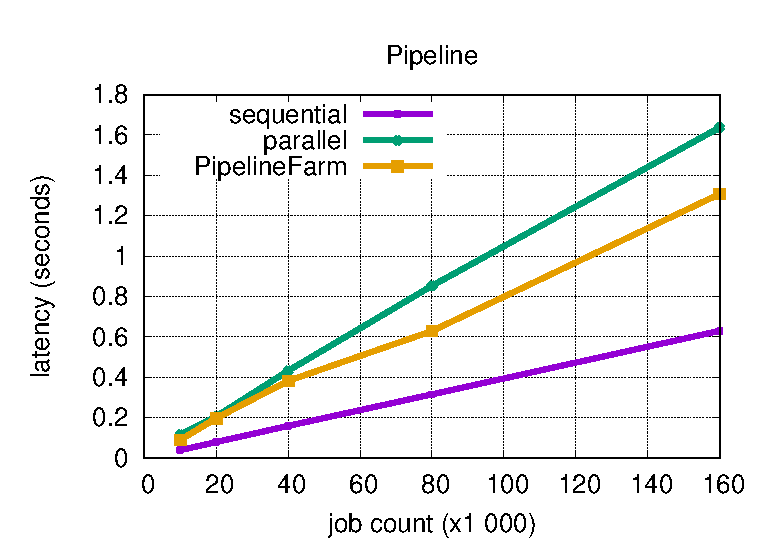
\includegraphics[width=0.265\textwidth]{plots/Pipeline.eps} & 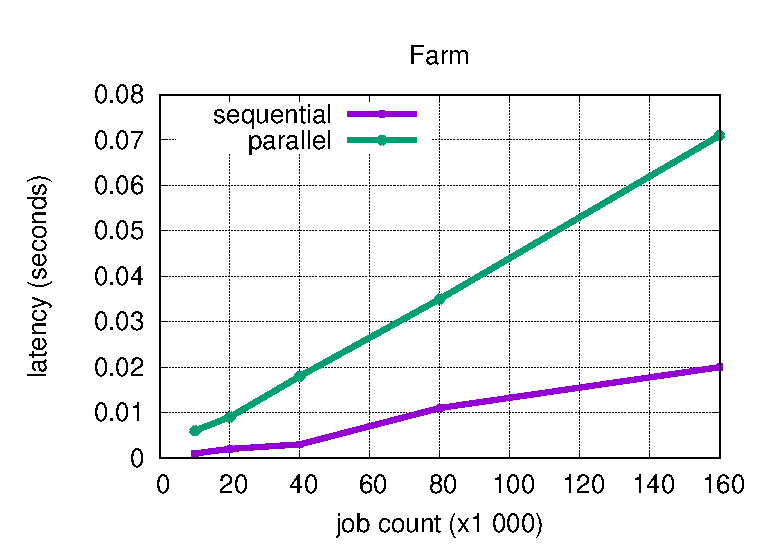
\includegraphics[width=0.265\textwidth]{plots/Farm.eps}\\
    \multicolumn{2}{c}{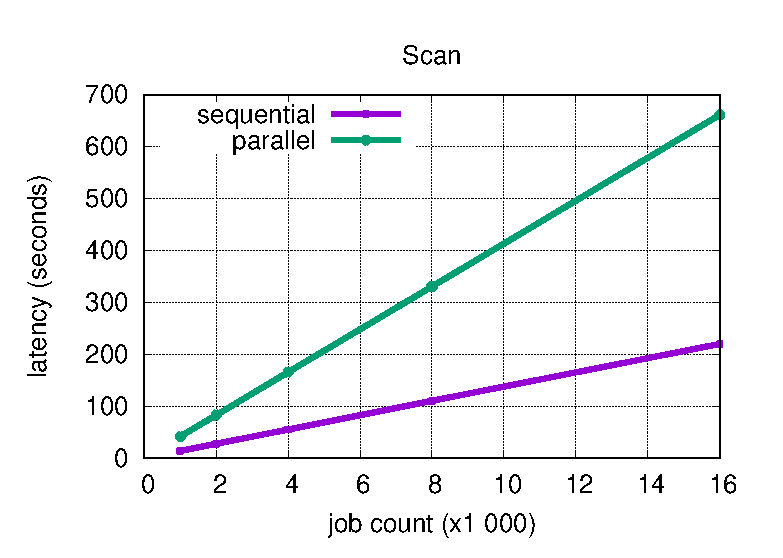
\includegraphics[width=0.265\textwidth]{plots/Scan.eps}}\\

    %(a) Map & (b) Reduce\\
    %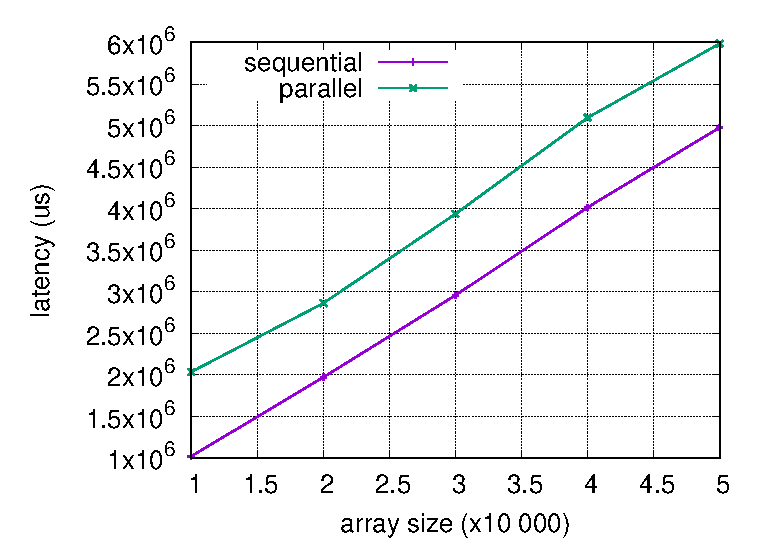
\includegraphics[width=0.25\textwidth]{plots/Map_heavy.eps} & 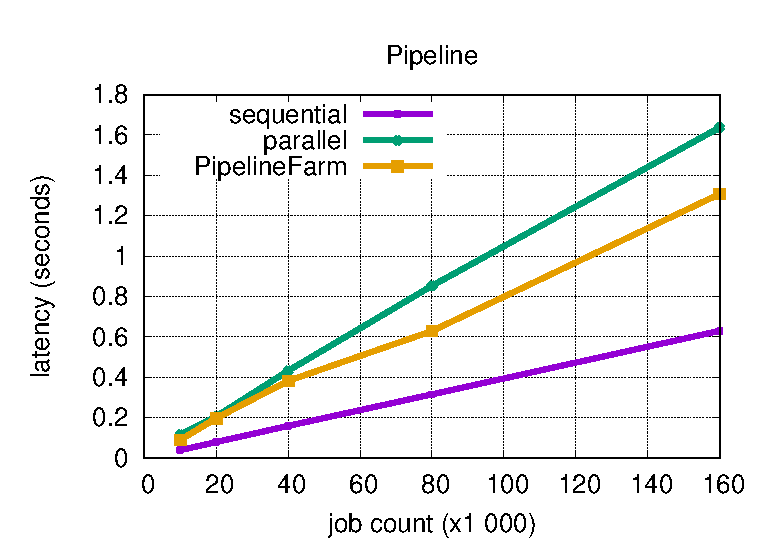
\includegraphics[width=0.25\textwidth]{plots/Pipeline.eps}\\
    %(a) MapHeavy & (b) Pipeline\\
   %\includegraphics[width=65mm]{it} &   \includegraphics[width=65mm]{it} \\
  %(c) third & (d) fourth \\[6pt]
  %\multicolumn{2}{c}{(e) fifth}
  \end{tabular}
\caption{Latency of the algorithms.} \label{latency}
\end{figure}

The Figure~\ref{latency} has the results obtained, for each algorithm, on the experiments.

Análise comparatória da performance dizendo porque correu bem e porque correu mal para cada um.
Análise geral, comparando a performance dos vaŕios uns cons os outros. Ex o map é o que aprenseta melhores resultados comparativamente à versão sequencial, bla bla
Podiamos medir a difenreça entre a paralela e a sequencial dividdo e assim tinhamos um valor que ea comparável com os outro salgoritmos

\section{Conclusion} \label{Conclusion}
After making this project we take some lessons with us. We now really understand that building parallel programs can be a very difficult task, serial implementations of a given pattern sometimes are just impossible to parallelize due to various dependencies along the code, so it is necessary to 'think out of the box' and create algorithms completely different from the serial ones.
This project was also quite different from the projects we are used to. We had to think like engineers: we had to debate and re-debate how we would implement our algorithms, we had to make some small 'sacrifices' in some areas (in our case memory) to achieve great results in other areas (time required), in other words, we had to reach a consensus on our priorities.
At the end of the day, we understood that parallel programming is essential when the amount of data to process is substantial and even more when efficiency is a must! 


\section*{Acknowledgments}

The authors would like to thank...

%https://www.gnu.org/software/libc/manual/html_node/CPU-Time.html para colocar na bibliografia


\section*{Comments}


% trigger a \newpage just before the given reference
% number - used to balance the columns on the last page
% adjust value as needed - may need to be readjusted if
% the document is modified later
%\IEEEtriggeratref{8}
% The "triggered" command can be changed if desired:
%\IEEEtriggercmd{\enlargethispage{-5in}}

% references section

% can use a bibliography generated by BibTeX as a .bbl file
% BibTeX documentation can be easily obtained at:
% http://mirror.ctan.org/biblio/bibtex/contrib/doc/
% The IEEEtran BibTeX style support page is at:
% http://www.michaelshell.org/tex/ieeetran/bibtex/
%\bibliographystyle{IEEEtran}
% argument is your BibTeX string definitions and bibliography database(s)
%\bibliography{IEEEabrv,../bib/paper}
%
% <OR> manually copy in the resultant .bbl file
% set second argument of \begin to the number of references
% (used to reserve space for the reference number labels box)
%\begin{thebibliography}{1}
%\bibitem{IEEEhowto:kopka}
%H.~Kopka and P.~W. Daly, \emph{A Guide to \LaTeX}, 3rd~ed.\hskip 1em plus
%  0.5em minus 0.4em\relax Harlow, England: Addison-Wesley, 1999.
%
%\end{thebibliography}

\bibliographystyle{IEEEtranS}
\bibliography{./IEEEabrv,bibliography}
%\bibliographystyle{./IEEEtran}
%\bibliography{./IEEEabrv,./IEEEexample}


% that's all folks
\end{document}
